\section{Deelvraag 2: Architectuur}
In deze paragraaf zijn de resultaten voor deelvraag 2 \textit{\SubquestionTwo} verzameld en geanalyseerd.
Er is samen met de architect van het CMS Erwin Keuning en met software engineer Kevin Snijder een IT architecture sketching sessie gedaan.
In deze sessie is de huidige softwarearchitectuur inbeeld gebracht en is er ook aandacht besteed aan het in beeld brengen van het datamodel.
Verder is er ook gebruik gemaakt van interne documentatie van het systeem om de tekeningen te ondersteunen.
De diagrammen zijn afgeleid van de originele tekeningen die gemaakt zijn tijdens de sessie deze tekeningen zijn te vinden in Bijlage \ref{appendix:ITArchitectureSketch}.

\subsection{Systeem}
Het eerste gedeelte van de IT architecture sketching is besteed aan het in beeld brengen van de huidige CMS, en hoe het interacteert met de huidige sites die Snakeware onderhoud.
Snakeware heeft op dit moment 3 verschillende modellen aan websites die ze onderhouden \gls{XSL}, Vue 2 en Vue 3.

\whitespace
De \gls{XSL} site is het oudste website model dat Snakeware nu onderhoud en maakt gebruik van de Snakeware Site code base.
Omdat origineel de \gls{XSL} sites er eerder was dan het \gls{CMS} was er des tijds voor gekozen om het van dezelfde Snakeware Site code base als basis te gebruiken.
% Dit heeft ervoor gezorgd dat het huidige \gls{CMS} aan te passen is met het \gls{CMS} (dit wordt alleen nooit gedaan).
De \gls{XSL} sites werken door middel van \gls{Stored procedures} om hun data op te halen en direct omzetten naar XML.
In figuur  \ref{fig:SystemArchitectureXSL} is te zien hoe de communicatie is tussen de verschillende systemen.
\todo[inline]{Voeg Stored procedures toe aan woordend lijst } 
% Het eerste gedeelte van het IT Architecuture sketching is besteed aan het globale systeem / flow van het systeem.
% Er zijn op dit moment 3 verschillende Snakeware Cloud site methodes deze methodes zijn \gls{XSL} \Parencite{XSL}, Vue 2 en Vue 3 \Parencite{Vue} site.
% De Vue 2 en 3 werken door middel van de Snakware Cloud API en de \gls{XSL} werkt door middel van de Snakeware.Site code base.
% In afbeelding \ref{fig:SystemArchitectureXSL} is te zien hoe de \gls{XSL} sites werken, in afbeeldingen \ref{fig:SystemArchitectureVue} is te zien hoe de vue sites werken.
%
% \whitespace
% Het Snakeware Cloud platform zelf is een \gls{XSL} site dat aangepast kan worden door middel van het CMS (dit wordt alleen nooit gedaan).
% Er wordt gebruik gemaakt van stored procedures om de data op te halen van de database, deze data wordt automatisch omgezet naar XML.
% De XML wordt getransformeerd in bruikbare JSON format \Parencite{JSON} in het geval van de Vue 2 en 3 sites, en in het geval van een \gls{XSL} site wordt het getransformeerd naar javascript en HTML \Parencite{HTML}.
% deze data wordt vervolgens gebruikt om de data te tonen op de frontend.
%

\whitespace
\begin{graphic}
	\captionsetup{type=figure}
    \caption{Globale systeemarchitectuur \gls{XSL} sites}
	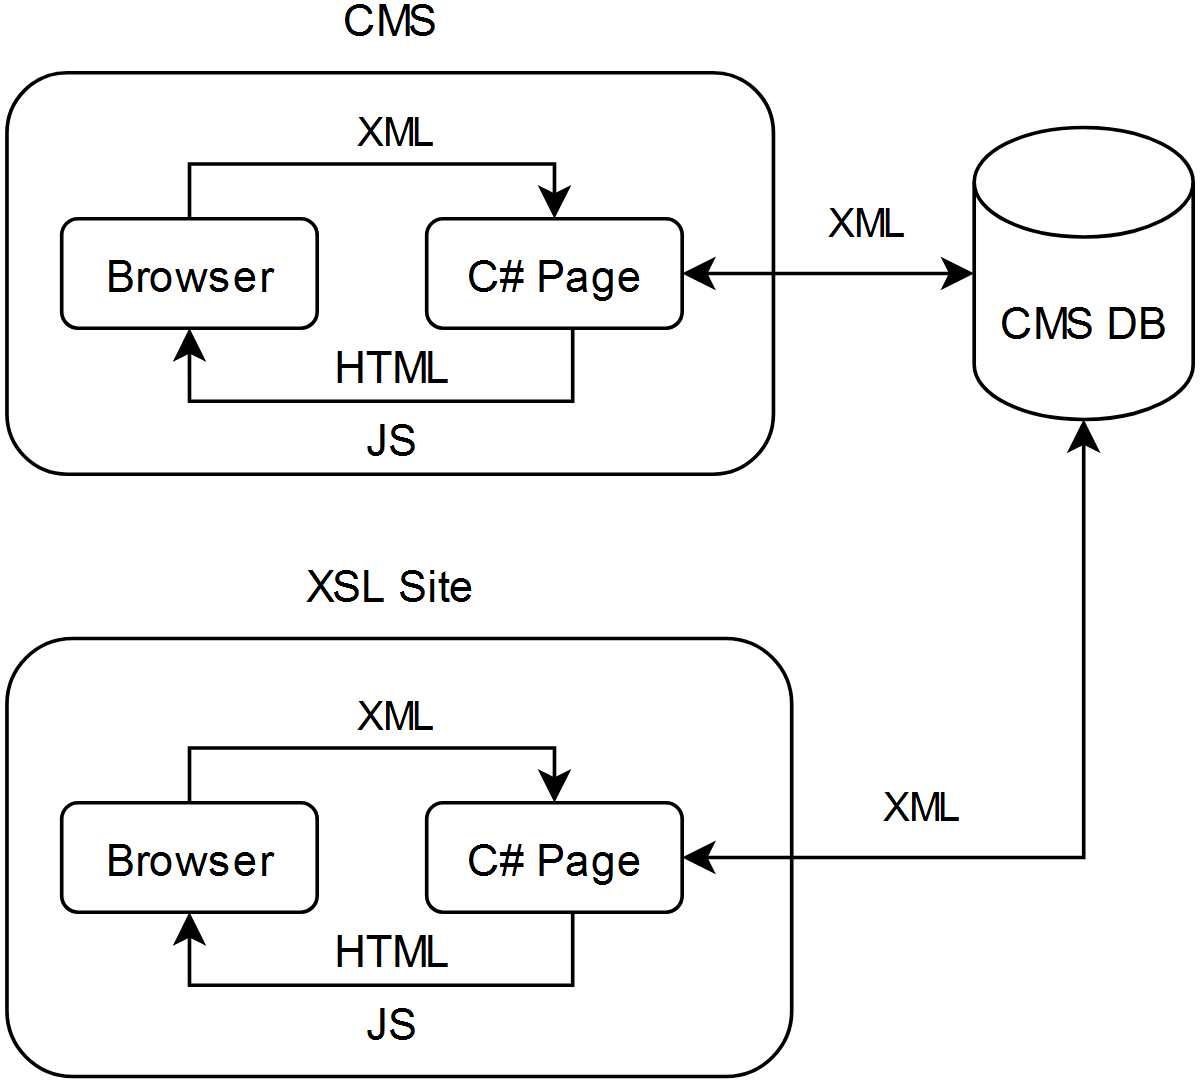
\includegraphics[scale=0.4]{XSLCMS}
	\label{fig:SystemArchitectureXSL}
\end{graphic}

\newpage

\whitespace
In het geval van de Vue sites wordt de XML omgezet naar het JSON format \parencite{JSON}.
Deze JSON wordt weer gebruikt om de correcte data te tonen op de frontend.
Een representatie van de flow van de Vue sites is te zien in figuur \ref{fig:SystemArchitectureVue}

\begin{graphic}
	\captionsetup{type=figure}
	\caption{Globale systeemarchitectuur Vue 2 en 3 sites}
    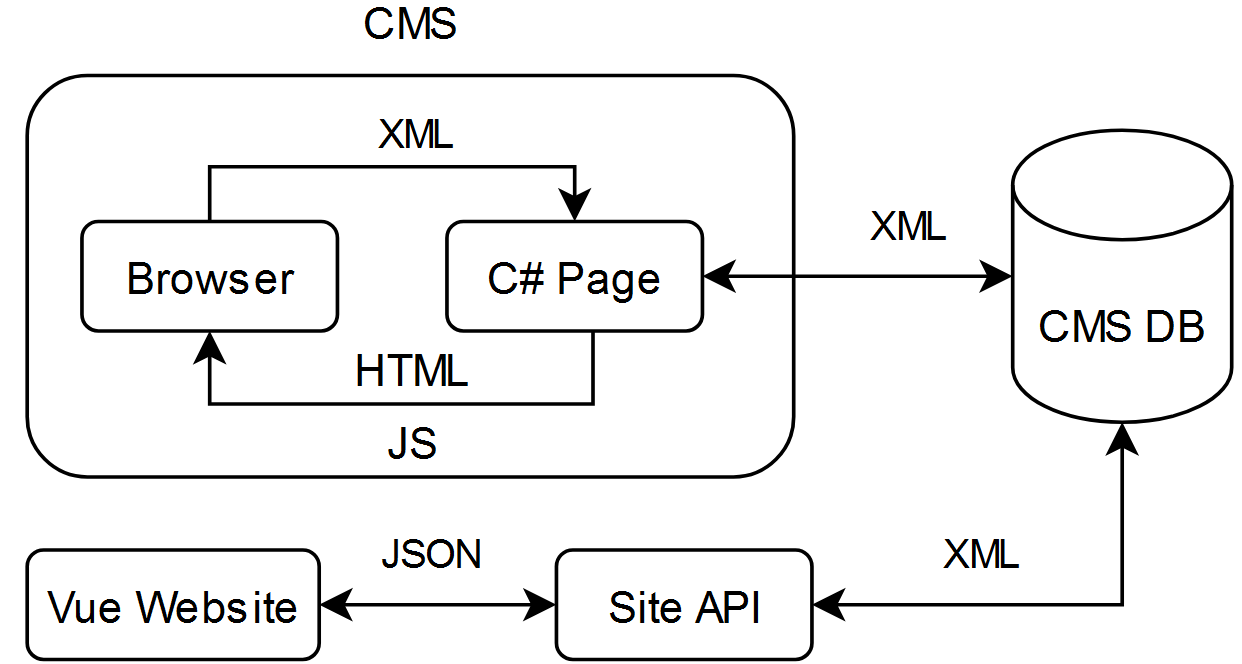
\includegraphics[scale=0.4]{VueCMS}
	\label{fig:SystemArchitectureVue}
\end{graphic}

% \todo[inline]{Ik had het ook nog even aan Stefan gevraagd en die zijn dat het prima is omdat het een representatie is van de tekeningen}

\whitespace
Tijdens de IT architecture sketching was er ook ruimte overgelaten om te onderzoeken waar er mogelijk verbeteringen gemaakt konden worden.
Uit de persoonlijke communicatie met Erwin en Kevin zijn de volgende punten uit gekomen.

\begin{itemize}
	\item[-]{Het Huidige \gls{CMS} maakt geen gebruik van de SOLID principes, dit zorgt er voor dat het moeilijk te testen en uit te breiden is van wege de interconnected code}
	\item[-]{Het \gls{CMS} is op dit moment een grote monoliet, dit brengt problemen met zich mee rond het schalen van het systeem.}
	\item[-]{Het is momenteel niet realistische om het \gls{CMS} te testen door middel van unit testen, dit is echter wel gewild.}
    \item[-]{Veel van de logica van het CMS zit vastgekoppeld in de frontend, en dit is niet gewild.}
\end{itemize}

\newpage
\subsection{Het datamodel}
\label{subsection:Datamodel}
Het volgende onderdeel is het schetsen van het datamodel, dit is ook gedaan samen met Erwin en Kevin.
Op dit moment maakt het \gls{CMS} gebruik van 288 tabellen, deze tabellen bevatten meerdere kolommen en zijn interconnected.
Daarom is er tijdens het schetsen van het datamodel alleen gekeken naar de belangrijkste tabellen en de relaties hier tussen.
De exacte data dat opgeslagen wordt in deze tabellen weggelaten om het overzichtelijk te houden.
Het versimpelde datamodel van het CMS is te zien in figuur \ref{fig:DatamodelCMS}.

\whitespace
\begin{graphic}
	\captionsetup{type=figure}
	\caption{Gesimplificeerde datamodel CMS}
	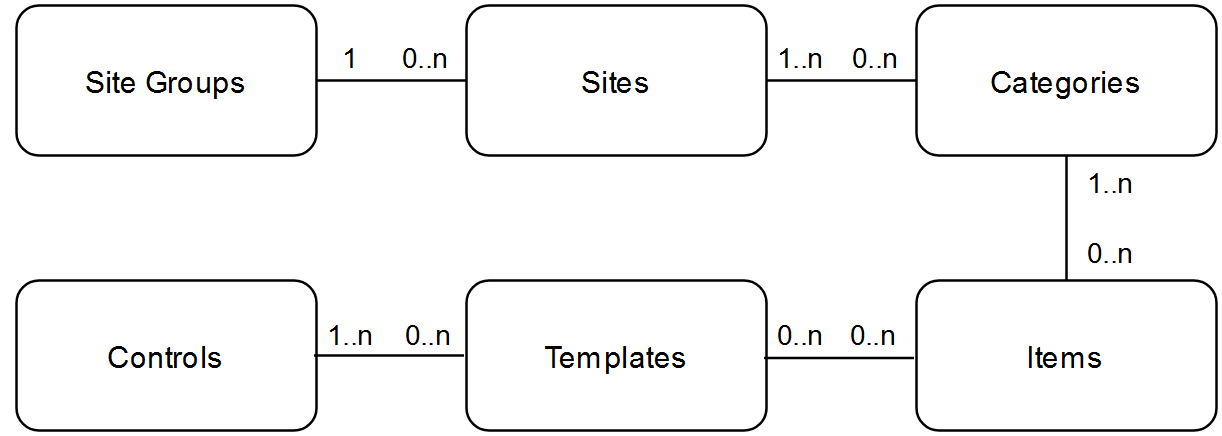
\includegraphics[scale=0.6]{CMSDatabaseModelB}
	\label{fig:DatamodelCMS}
\end{graphic}

\whitespace[2]
Na het schetsen van het datamodel is er gevraagd waar op dit moment de meeste problemen worden gevonden in het datamodel.
Deze punten zijn verzameld tijdens de sessie door middel van persoonlijke communicatie met Erwin en Kevin.
\begin{itemize}
    \item[-]{Het datamodel is erg complex, dit maakt het lastig om nieuwe functionaliteiten in het CMS te bouwen}
    \item[-]{Het datamodel heeft te veel connecties met andere tabellen terwijl dit niet nodig zou moeten zijn.
        Dit maakt het systeem onnodig complex.}
    \item[-]{De huidige naamgeving van de tabellen en kolommen is niet als gewild.
            Als dit nu aangepast zou worden zou dit voor veel problemen opleveren in de code, maar met een nieuw project is het gewild dat er een andere naamgeving wordt gebruikt.}
\end{itemize} 
% \todo[inline]{dit denk ik weg halen}
% Tijdens de sessie kwam er naar voren dat mensen binnen het R\&D uitgesproken meningen hebben over een nieuw datamodel.
% Hierom wordt er tijdens de ontwerpfase met het R\&D team een sessie gepland om ideeen te leveren voor een nieuw data model.
% Deze input zal gebruikt worden om het datamodel te ontwerpen.
%

\subsection{Antwoord en resultaat}
Samen met Erwin Keuning en Kevin Snijder zijn er door middel van IT architecture sketching 2 systeem schetsen gemaakt (zie figuur \ref{fig:SystemArchitectureXSL} en \ref{fig:SystemArchitectureVue})
Door middel van deze tekening is het huidige systeem en datamodel in beeld gebracht.
Daarnaast zijn er door de gesprekken met Erwin en Kevin de volgende randvoorwaarden opgesteld.

\begin{itemize}
    \item[-]{Het eind product moet voldoende documentatie bevatten.}
    \item[-]{De code moet voldoen aan huidige coderingsstandaarden}
    \item[-]{De code moet getest worden door middel van verschillende test methodes}
    \item[-]{De code zal geschreven worden in programmeertalen die gebruikt worden binnen Snakeware}
\end{itemize}

